\documentclass[aspectratio=169, 13pt, t]{beamer}

	\usepackage[english, russian]{babel}
	\usepackage[utf8]{inputenc}
	
	\usepackage{graphicx}
	\usepackage{sidecap}
	\usepackage{mathtools}
	\usepackage{appendixnumberbeamer}
	\usepackage{bbm}
	\usepackage{tcolorbox}
	
	\newcommand{\sbrkt}[1]{\left[ #1 \right]}
	\DeclarePairedDelimiter\bra{\langle}{\rvert}
	\DeclarePairedDelimiter\ket{\lvert}{\rangle}
	\DeclarePairedDelimiterX\braket[2]{\langle}{\rangle}{#1 \delimsize\vert #2}
	\newcommand{\rbrkt}[1]{\left( #1 \right)}
	\newcommand{\lbrkt}[1]{\left< #1 \right>}
	\newcommand{\diff}{\,\mathrm{d}} 	
	
	\makeatletter
	\newcommand\supervisor[1]{\def\@supervisor{{Supervisor: #1}}}
	\makeatother
	
	\graphicspath{{./Pics/}{../Pictures/}}
	\usetheme{mipt_beamer}
	\usefonttheme[onlymath]{serif}

\title{Coherent josephson qubit suitable for scalable quantum integrated circuits (2013) \\~\\Superconducting quantum circuits at the surface code threshold for fault tolerance (2014)}
\author{\large \textit{\textbf{ИКС}}}
\date{\today}

\setlength{\jot}{15pt}
\setbeamertemplate{footline}[page number]
\renewcommand*{\inserttotalframenumber}{\insertpresentationendpage}
\newcommand{\Tr}[1]{\text{Tr}\left[#1\right]}


\newtcolorbox{mybox}[1][]{
colback=white,
colbacktitle=white,
colframe=miptblue,
boxrule=1pt,
titlerule=0pt,
arc=15pt,
}

\begin{document}
  
{
\begin{frame}[plain]
  \titlepage
\end{frame}
}


\AtBeginSection[] {
\frame[plain] {
	\begin{columns}[c]
	\column{0.7\textwidth}    
	    \tableofcontents[currentsection]
	\column{0.3\textwidth}
		\centering
		\hspace{-2cm}\includegraphics[width=0.9\textwidth]{2xmons}
		
    	\vspace*{1cm}
    	\hspace{-2cm}\includegraphics[width=0.9\textwidth]{xmons}

  	\end{columns}
}
	\addtocounter{page}{-1}

}


\section{Coherent josephson qubit...}
\subsection{Общий вид}
\begin{frame}[t]\frametitle{\secname}\framesubtitle{\subsecname}

\begin{columns}[c]
\column{0.65\textwidth}
\centering
\includegraphics[width=\textwidth]{xmon}
\column{0.35\textwidth}
Одноостровной трансмон на основе двух копланарных волноводов
\begingroup
\setlength{\abovedisplayskip}{0pt} \setlength{\abovedisplayshortskip}{0pt}
\setlength{\belowdisplayskip}{0pt} \setlength{\belowdisplayshortskip}{0pt}
\begin{align*}
C_q &\approx 100 \text{ фФ}\\
E_C &\approx -\alpha \approx 200 \text{ МГц}\\
E_J &\approx 95 E_C\\
\nu_{ge} &\approx 6 \text{ ГГц}
\end{align*}
\endgroup
Резонаторы $\lambda/4$ с ВШК на разомкнутом конце, $Q_l \sim 10^4$
\end{columns}

\end{frame}

\begin{frame}[t]\frametitle{\secname}\framesubtitle{\subsecname}
Схема конутра для квантования системы

\vspace{.5cm}
\begin{columns}[c]
\column{\textwidth}
\centering
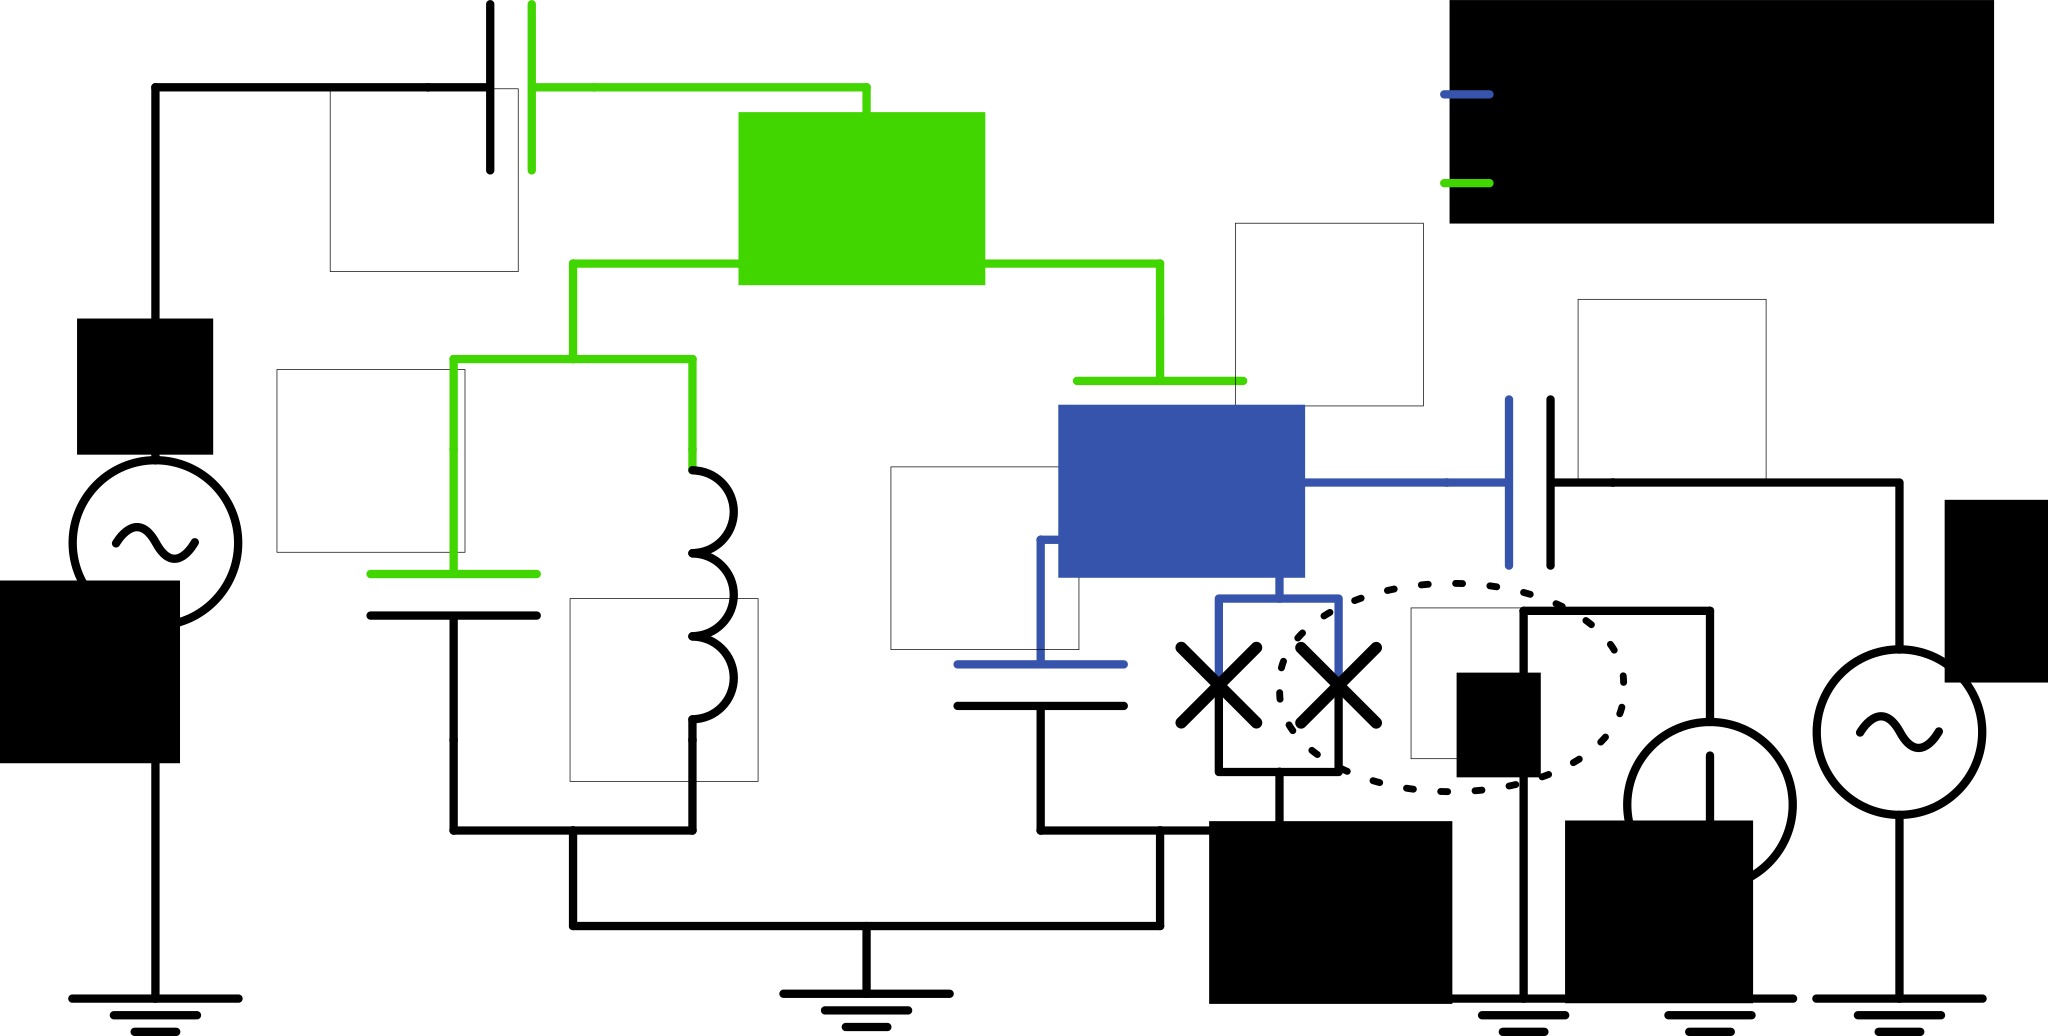
\includegraphics[height=0.6\textheight]{xmon-resonator}
\end{columns}

\end{frame}

\subsection{Эволюция конфигурации}
\begin{frame}[t]\frametitle{\secname}\framesubtitle{\subsecname}

В основном прогресс во времени жизни кубита обязан оптимизации его геометрии:

\centering
\includegraphics[height=0.75\textheight]{perspective}

\end{frame}

\begin{frame}[t]\frametitle{\secname}\framesubtitle{\subsecname}
Различные конфигурации петли для подачи МП на сквид иксмона:

\vspace{.2cm}
\centering
\includegraphics[height=0.75\textheight]{perspective2}

\end{frame}

\subsection{Когерентность}
\begin{frame}[c]\frametitle{\secname}\framesubtitle{\subsecname}
\begin{columns}[c]
\column{0.5\textwidth}
\centering
\includegraphics[height=0.9\textheight]{coherence}
\column{.5\textwidth}
Некоторые расчетные и измеренные параметры когерентности:
\begin{align*}
T_1^C &\sim 0.3\text{ мс} \\
T_1^M &\sim 30\text{ мс} \\
T_1 &\leq 44 \text{ мкс} \\
T_2^* &\leq 15 \text{ мкс} < T_1/2  
\end{align*}
\end{columns}
\end{frame}


\subsection{Некогерентные дефекты}
\begin{frame}[t]\frametitle{\secname}\framesubtitle{\subsecname}
\centering
\includegraphics[height=0.6\textheight]{defect_sim}

\[
\frac{\partial}{\partial t}\hat \rho_{qd} = \frac{i}{\hbar}\left[\hat\rho_{qd},\mathcal{\hat H}_{qd}\right] - \sum_i \Gamma_i \mathcal{D}[\mathcal{\hat O}_i]\hat \rho_{qd} \Rightarrow \Gamma_1 = \frac{2g^2\Gamma_\Sigma}{\Gamma_\Sigma^2 + \Delta^2}+\Gamma_{1q}
\]
\end{frame}

\begin{frame}[c]\frametitle{\secname}\framesubtitle{\subsecname}
\begin{columns}[c]
\column{0.6\textwidth}
\centering
\includegraphics[width=0.9\textwidth]{defectsT1}
\column{.4\textwidth}
\centering
\includegraphics[width=\textwidth]{defectsT12}

\includegraphics[width=0.8\textwidth]{defect_pos}
\end{columns}
\end{frame}

\section{Superconducting circuits...}
\subsection{Образец}
\begin{frame}[c]\frametitle{\secname}\framesubtitle{\subsecname}
\centering
\includegraphics[height=0.8\textheight]{scheme}
\end{frame}

\begin{frame}[c]\frametitle{\secname}\framesubtitle{\subsecname}
\centering
\includegraphics[height=0.85\textheight]{xmons_photo}
\end{frame}

\subsection{Установка}
\begin{frame}[c]\frametitle{\secname}\framesubtitle{\subsecname}
\centering
\includegraphics[height=0.85\textheight]{cryo}
\end{frame}

\subsection{Стохастическое оценивание вентилей}
\begin{frame}[c]\frametitle{\secname}\framesubtitle{\subsecname}
\centering
\includegraphics[width=0.65\textwidth]{rb}

\end{frame}

\subsection{Контролируемый вентиль фазы}

\begin{frame}[t]\frametitle{\secname}\framesubtitle{\subsecname}
\centering
\includegraphics[width=0.9\textwidth]{cz}

\includegraphics[height=0.48\textheight]{detune}
\includegraphics[height=0.5\textheight]{czrb}
\end{frame}

\subsection{Формирование GHZ-состояний}
\begin{frame}[t]\frametitle{\secname}\framesubtitle{\subsecname}
\includegraphics[width=\textwidth]{ghz}

\[
\text{Fidelity} = \text{Tr}[\hat\rho\hat\rho_{ideal}]
\]
\end{frame}

\section*{}
\subsection*{Заключение}
\begin{frame}[c]\frametitle{\secname}\framesubtitle{\subsecname}
\begin{columns}[c]
\column{0.5\textwidth}
\begin{itemize}
\item Простота геометрии и аккуратный расчет дают большой выигрыш во времени жизни. Основными лимитирующими факторами остаются двухуровневые дефекты и, вероятно, квазичастицы
\item Сверхпроводящими кубитами возможно управлять с большой точностью при помощи оптимизации импульсов, что позволит в будущем применять коды, исправляющие ошибки
\end{itemize}
\column{0.5\textwidth}
\centering

\includegraphics[width=\textwidth]{errcorr}
\end{columns}

\end{frame}

\end{document}